\documentclass[uplatex,11pt]{jsarticle}
\usepackage{type1ec}
\usepackage[OT2,T1]{fontenc}
\usepackage[russian,english,japanese]{babel}
\usepackage{wrapfig}
\usepackage[dvipdfmx]{graphicx}
\begin{document}
\subsection*{常盤台ロシア語学校(仮称) 不定期通信7}
\begin{flushright}
  2018-07-27
\end{flushright}
\subsubsection*{今後の開講予定}
\begin{itemize}
  \item 春学期は2018-08-03(金)まで開講します.
  \item 夏休み期間中は要望に応じて開講します. (8/15~8/18と8/25, 8/27~9/20は不可)
  \item 秋学期の初め頃に秋学期の開講日時のアンケートを設置します.
\end{itemize}
\subsubsection*{PC・Macによるロシア語入力の方法}
\begin{description}
  \item[Windows 10]\mbox{}\selectlanguage{russian}\\
    設定→時刻と言語→地域と言語→言語を追加する よりRusski{i0}を選択 \\
    ※設定→アプリ→アプリと機能→オプション機能の管理→機能の追加 より「ヨーロッパ各国語追加フォント」をインストールしておくと文書作成時に有用かもしれません.
\selectlanguage{english}
  \item[Macintosh]\mbox{}\\
    macOS Sierra: 入力ソースを使用してほかの言語で入力する \\
    https://support.apple.com/kb/PH25311
\end{description}
\selectlanguage{russian}
ロシア語のキー配列は{I0}CUKEN配列(※別紙参照)といって
\selectlanguage{english}
QWERTY配列とは異なる並び(発音という観点から見て)なので、スムースな入力には慣れが必要です. (記号の並びも日本語キーボードとは一部異なります) \\
Google翻訳やYandex Translateでは前述の設定を行わなくとも入力ツール(入力欄にアイコンがあります)から
\selectlanguage{russian}
{I0}CUKEN配列のキーボードを利用することが出来るので、練習に便利です.
\begin{wrapfigure}[7]{R}[0cm]{8cm}
\centering
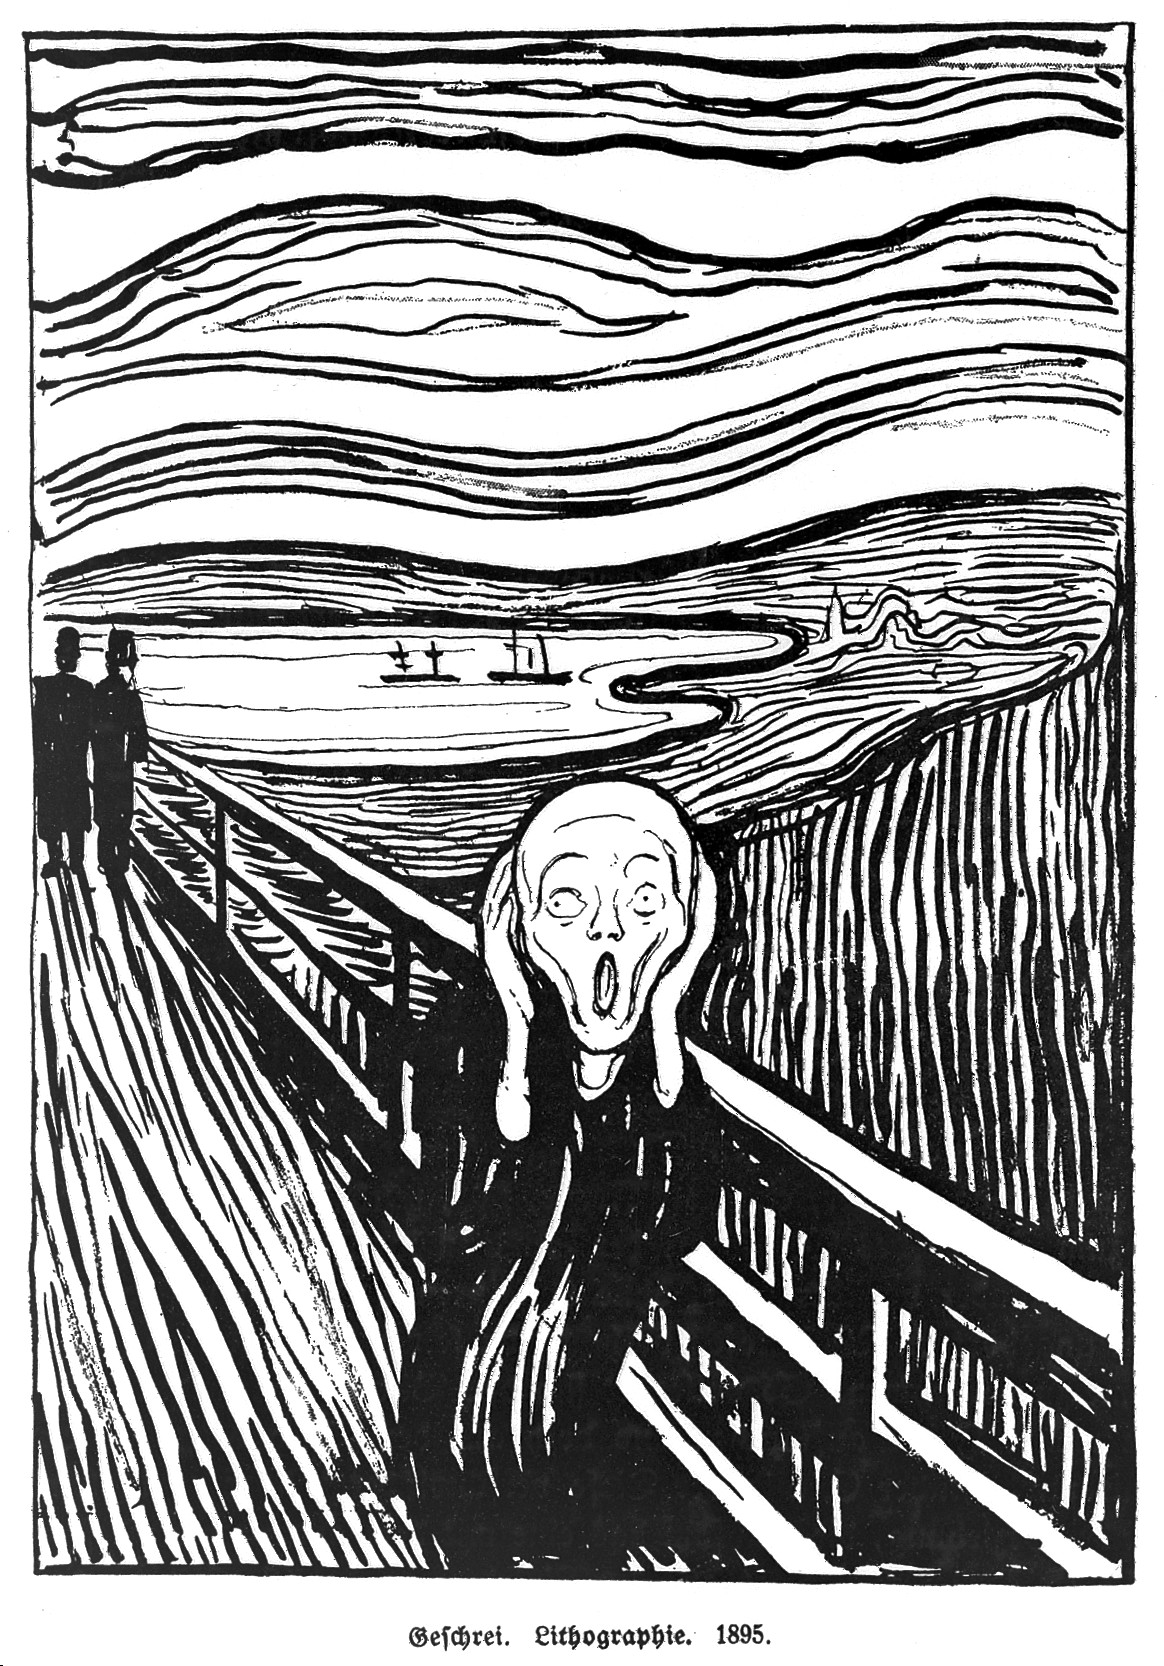
\includegraphics[width=30mm,bb=0 0 279 400]{_The_scream_._Wellcome_L0011212.jpg}
\caption{\flqq{}Krik\frqq}
\end{wrapfigure}
\subsubsection*{先週・今週のフレーズ}
\noindent
"--* Poqem\'u vy kriq\'ite? \\
"--* あなたは何故叫んでいるのですか? \\
\\
"--* Sqastl\'ivogo put\'i! \\
"--* 道中ご無事で! \\
\\
単語: kriq\'at{p1} 叫ぶ, ris\'unok 絵, sqastl\'ivy{i0} 幸運な
\end{document}
